%-----------------------------------------------------------------------------%
\chapter{\babEnam}
%-----------------------------------------------------------------------------%
\todo{tambahkan kata-kata pengantar bab 6 disini}

\section{Usecase Diagram}

\subsection{As Is Usecase Diagram}

\subsection{To Be Usecase Diagram}

\begin{figure}
	\centering
	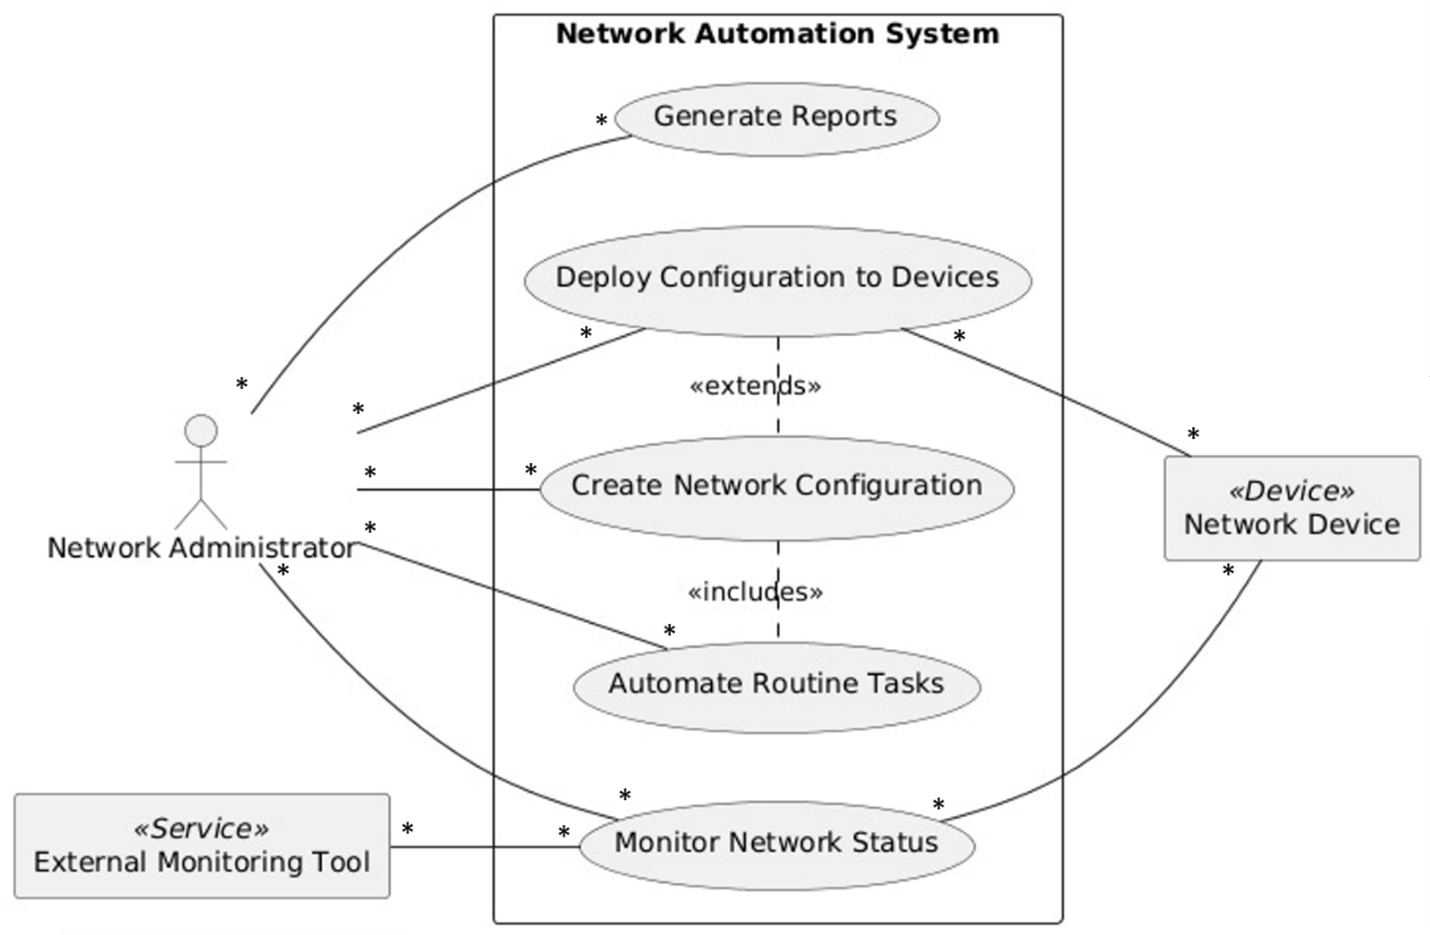
\includegraphics[width=0.70\textwidth]
		{assets/pics/usecase_diagram.png}
	\caption{Usecase diagram}
	\label{fig:usecase_diagram_ucp}
\end{figure}


\subsection{Actors}
\begin{itemize}
    \item \textbf{Network Administrator}: The primary user of the system who can perform various network management tasks.
    \item \textbf{External Monitoring Tool}: A service used to monitor the status of the network, which interacts with the system.
\end{itemize}

\subsection{System}
\textbf{Network Automation System}: The main system used by network administrators to manage configurations, automate tasks, and monitor the network status.

\subsection{Use Cases}
\begin{itemize}
    \item \textbf{Create Network Configuration}: Network administrators can create new network configurations using the system.
    \item \textbf{Automate Routine Tasks}: Routine network tasks can be automated as part of the network configuration process.
    \item \textbf{Deploy Configuration to Devices}: Once a configuration is created, the system can deploy it across network devices. This use case extends \textit{Create Network Configuration}.
    \item \textbf{Generate Reports}: Network administrators can generate reports from the system based on collected data or actions taken.
    \item \textbf{Monitor Network Status}: The system allows real-time monitoring of network status by the administrator, with the \textit{External Monitoring Tool} also involved in this process.
\end{itemize}

\subsection{Relationships}
\begin{itemize}
    \item \textbf{Network Administrator} has direct associations with all use cases within the system.
    \item The \textbf{Network Automation System} is connected to \textit{Network Devices} that receive configurations deployed by the system.
    \item The system is also connected to the \textit{External Monitoring Tool}, which assists in monitoring network status.
\end{itemize}


\section{Use Case Descriptions}

\subsection{Create Network Configuration}


\begin{table}[H]
    \centering
    \caption{Usecase Description Create Network Configuration}
    \renewcommand{\arraystretch}{1.3}
    \begin{tabular}{|p{3cm}|p{11cm}|}
        \hline
        \textbf{Use Case} & \textbf{Create Network Configuration} \\
        \hline
        \textbf{Actor} & Network Administrator \\
        \hline
        \textbf{Description} & Network Administrator creates configurations for network devices, including IP settings, routing protocols, and security parameters. \\
        \hline
        \textbf{Preconditions} & 
        \begin{itemize}
            \item Network Automation System is running.
            \item The user is authenticated and has permissions to create configurations.
        \end{itemize} \\
        \hline
        \textbf{Postconditions} & A network configuration is successfully created and ready to be deployed to devices. \\
        \hline
        \textbf{Trigger} & Administrator starts a configuration process. \\
        \hline
        \textbf{Main Flow} & 
        \begin{itemize}
            \item The Network Administrator selects the option to create a new configuration.
            \item The system prompts the user for device parameters.
            \item The user enters necessary details.
            \item The system generates the configuration based on the input.
            \item The configuration is saved in the system.
        \end{itemize} \\
        \hline
        \textbf{Alternative Flow} & If there is a validation error during data entry, the system prompts the user to correct the input. \\
        \hline
        \textbf{Includes} & Automate Routine Tasks \\
        \hline
    \end{tabular}
\end{table}

\subsection{Deploy Configuration to Devices}


\begin{table}[H]
    \centering
    \caption{Usecase Description Deploy Configuration to Devices}
    \renewcommand{\arraystretch}{1.3}
    \begin{tabular}{|p{3cm}|p{11cm}|}
        \hline
        \textbf{Use Case} & \textbf{Deploy Configuration to Devices} \\
        \hline
        \textbf{Actor} & Network Administrator \\
        \hline
        \textbf{Description} & Deploys the created configuration to network devices (e.g., routers, switches). \\
        \hline
        \textbf{Preconditions} & 
        \begin{itemize}
            \item A network configuration exists.
            \item The Network Administrator has access to the devices.
        \end{itemize} \\
        \hline
        \textbf{Postconditions} & Devices are configured with the new settings. \\
        \hline
        \textbf{Trigger} & Administrator initiates the deployment process. \\
        \hline
        \textbf{Main Flow} & 
        \begin{itemize}
            \item The administrator selects the configuration to deploy.
            \item The system validates device accessibility.
            \item The configuration is pushed to the devices.
            \item The system confirms successful deployment.
        \end{itemize} \\
        \hline
        \textbf{Alternative Flow} & If a device is not reachable, the system logs an error and notifies the administrator. \\
        \hline
        \textbf{Extends} & Create Network Configuration \\
        \hline
    \end{tabular}
\end{table}

\subsection{Monitor Network Status}


\begin{table}[H]
    \centering
    \caption{Usecase Description Monitor Network Status}
    \renewcommand{\arraystretch}{1.3}
    \begin{tabular}{|p{3cm}|p{11cm}|}
        \hline
        \textbf{Use Case} & \textbf{Monitor Network Status} \\
        \hline
        \textbf{Actor} & Network Administrator, External Monitoring Tool (Service) \\
        \hline
        \textbf{Description} & Monitors the status of network devices, ensuring their operational health and performance. \\
        \hline
        \textbf{Preconditions} & Devices are accessible. \\
        \hline
        \textbf{Postconditions} & The administrator is aware of the current network status and any potential issues. \\
        \hline
        \textbf{Trigger} & Monitoring occurs periodically or when triggered by the administrator. \\
        \hline
        \textbf{Main Flow} & 
        \begin{itemize}
            \item The system polls devices for their current status.
            \item Results are displayed to the administrator.
            \item Alerts are generated if issues are detected.
        \end{itemize} \\
        \hline
        \textbf{Alternative Flow} & If a device is down, the system logs the issue and notifies the administrator. \\
        \hline
        \textbf{External Service Interaction} & Integrates with external monitoring tools for enhanced monitoring. \\
        \hline
    \end{tabular}
\end{table}

\subsection{Automate Routine Tasks}


\begin{table}[H]
    \centering
    \caption{Usecase Description Automate Routine Tasks}
    \renewcommand{\arraystretch}{1.3}
    \begin{tabular}{|p{3cm}|p{11cm}|}
        \hline
        \textbf{Use Case} & \textbf{Automate Routine Tasks} \\
        \hline
        \textbf{Actor} & Network Administrator \\
        \hline
        \textbf{Description} & Automates routine network tasks, such as scheduled configuration backups, device reboots, or performance checks. \\
        \hline
        \textbf{Preconditions} & Network devices are operational. \\
        \hline
        \textbf{Postconditions} & Routine tasks are executed as scheduled. \\
        \hline
        \textbf{Trigger} & Scheduled by the system or manually initiated by the administrator. \\
        \hline
        \textbf{Main Flow} & 
        \begin{itemize}
            \item The system executes predefined tasks automatically.
            \item Results are logged and displayed to the administrator.
        \end{itemize} \\
        \hline
        \textbf{Alternative Flow} & If a task fails, the system logs an error and retries the task. \\
        \hline
    \end{tabular}
\end{table}

\subsection{Generate Reports}


\begin{table}[H]
    \centering
    \caption{Usecase Description Generate Reports}
    \renewcommand{\arraystretch}{1.3}
    \begin{tabular}{|p{3cm}|p{11cm}|}
        \hline
        \textbf{Use Case} & \textbf{Generate Reports} \\
        \hline
        \textbf{Actor} & Network Administrator \\
        \hline
        \textbf{Description} & Generates reports on network performance, status, and any configuration changes made. \\
        \hline
        \textbf{Preconditions} & Data must be available from network monitoring or configuration changes. \\
        \hline
        \textbf{Postconditions} & A report is generated and available for review. \\
        \hline
        \textbf{Trigger} & Administrator requests a report or the system generates one on schedule. \\
        \hline
        \textbf{Main Flow} & 
        \begin{itemize}
            \item The administrator selects the type of report to generate.
            \item The system gathers relevant data.
            \item The report is generated and displayed or emailed to the administrator.
        \end{itemize} \\
        \hline
    \end{tabular}
\end{table}
